\documentclass[11pt]{article}
\usepackage{epsfig, mdwlist, amssymb}
\usepackage{fullpage}
%\usepackage{color}
\usepackage{url}
\usepackage{natbib}
%%\usepackage{emulateapj}
%\usepackage{footnote}
\usepackage{deluxetable}

\newcommand{\oii}{[O~{\sc ii}]}
\newcommand{\oiii}{[O~{\sc iii}]}
\newcommand{\nii}{[N~{\sc ii}]}
\newcommand{\sii}{[N~{\sc ii}]}
\newcommand{\hei}{He~{\sc i}}
\newcommand{\simt}{{\tt simulate-templates.py}}

\newcommand{\oiilam}{[O~{\sc ii}]~\ensuremath{\lambda\lambda3726,29}}

\newcommand{\kms}{km~s$^{-1}$}

\newcommand{\apj}{ApJ}
\newcommand{\pasp}{PASP}
\newcommand{\apjs}{ApJS}
\newcommand{\TODO}[1]{{\it \color{red} (#1)}}

\begin{document}
\title{Simulating State-of-the-Art Spectral Templates for DESI} 

\author{John Moustakas (Siena College)}
\maketitle

%\abstract{ This technote documents the construction of the preliminary
%  (currently v1.2) emission-line galaxy (ELG) templates for DESI.  }

\section{Introduction}

This document describes the methodology and code which was developed to generate
one-dimensional, noiseless, high-resolution spectral templates for DESI.  The
initial focus of this effort has been on emission-line galaxies (ELG), luminous
red galaxies (LRG), bright-galaxy survey galaxies (BGS), and stars (STAR), but
eventually quasars (QSO), including Ly$\alpha$-QSOs, and standard stars (STD)
will be supported.

The models are based on a combination of empirical constraints (i.e.,
spectroscopy and photometry of galaxies and quasars over a broad redshift range)
and state-of-the-art theoretical models.  These templates have a myriad of
applications, but will be used primarily to help develop and optimize the
end-to-end DESI spectroscopic pipeline (``data challenges'')---from raw data to
redshifts and final spectral classifications---as well as to help develop and
validate various target-selection strategies.

All the code described below, as well as the text of this document and the code
used to generate the figures are maintained in the public DESI {\tt Github}
repository {\tt
  desihub/desisim}\footnote{\url{https://github.com/desihub/desisim}} under the
{\tt py/desisim} and {\tt doc/tex/simulate-templates} directories, respectively.

%ToDo:
%* Allow AGN-like emission-line ratios.
%* Add (weak) emission lines to the LRG templates.
%* Fix the random seed so the spectrum results are reproducible.
%* Add units tests.
%* Add nebular continuum to the EMSpectrum class.
%* The empirical coefficients in EMSpectrum are hard-coded.
%* Add more emission lines.

\section{Getting Started Quickly}

This section presents several high-level examples so that you can get started
building templates quickly.  To install the software and its dependencies please
carefully review Appendix~\ref{sec:install}.  

The only mandatory input required by \simt{} is to specify the number of
templates/models via the {\tt nmodel} input and, optionally, the object type
(although the default is {\tt ELG}); the code is initialized with sensible
defaults for all the other optional inputs.  For example, to generate 100 {\tt
  ELG} spectra, type

\begin{verbatim}
% simulate-templates.py --nmodel 100
\end{verbatim}




\begin{verbatim}

usage: simulate-templates.py [-h] [--nmodel] [--objtype] [--minwave]
                             [--maxwave] [--cdelt] [--nocolorcuts]
                             [--notemplates] [--noplot] [--outfile] [--qafile]
                             [--zrange-elg ] [--rmagrange-elg ] [--minoiiflux]
                             [--zrange-lrg ] [--zmagrange-lrg ]
                             [--zrange-bgs ] [--rmagrange-bgs ]

Simulate noiseless, infinite-resolution spectral templates for DESI.

optional arguments:
  -h, --help         show this help message and exit
  --nmodel           number of model (template) spectra to generate (required
                     input) (default: None)
  --objtype          object type (ELG, LRG, QSO, BGS, STD, or STAR) (default:
                     ELG)
  --minwave          minimum output wavelength range [Angstrom] (default:
                     3600)
  --maxwave          maximum output wavelength range [Angstrom] (default:
                     10000)
  --cdelt            dispersion of output wavelength array [Angstrom/pixel]
                     (default: 2)
  --nocolorcuts      do not apply color cuts to select objects (only used for
                     object types ELG, LRG, and QSO) (default: False)
  --notemplates      do not generate templates (but do generate the diagnostic
                     plots if OUTFILE exists) (default: False)
  --noplot           do not generate diagnostic (QA) plots (default: False)
  --outfile          output FITS file name (default: OBJTYPE-templates.fits)
  --qafile           output file name for the diagnostic (QA) plots (default:
                     OBJTYPE-templates.pdf)

options for objtype=ELG:
  --zrange-elg       minimum and maximum redshift (default: (0.6, 1.6))
  --rmagrange-elg    Minimum and maximum r-band (AB) magnitude range (default:
                     (21.0, 23.5))
  --minoiiflux       Minimum integrated [OII] 3727 flux (default: 1E-17)

options for objtype=LRG:
  --zrange-lrg       minimum and maximum redshift (default: (0.5, 1.1))
  --zmagrange-lrg    Minimum and maximum z-band (AB) magnitude range (default:
                     (19.5, 20.6))

options for objtype=BGS:
  --zrange-bgs       minimum and maximum redshift (default: (0.01, 0.4))
  --rmagrange-bgs    Minimum and maximum r-band (AB) magnitude range (default:
                     (15.0, 19.0))

\end{verbatim}


\subsection{Building Templates for Other Object Types}

In general, building 



What about stars?!

\section{The Details}

The following sections describe each specific DESI spectral class in more
detail, as well as various planned (and unplanned) avenues for improving the
models.

%\section{Building a Realistic Emission-Line Spectrum}

\subsection{ELGs}

\begin{figure}
\centering
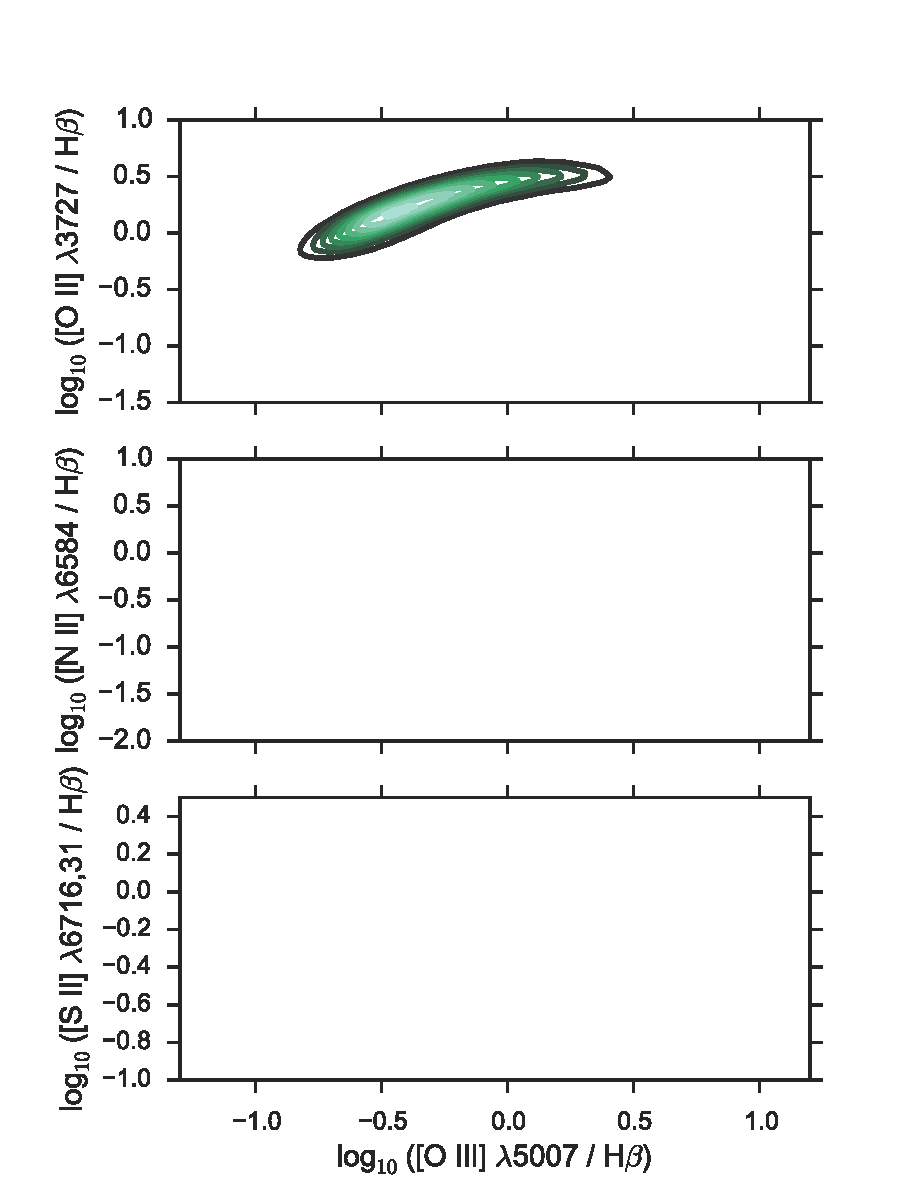
\includegraphics[width=0.8\textwidth]{figures/oiiihb.pdf}
\caption{Caption. \label{fig:oiiihb}}
\end{figure}

%DESI aims to measure redshifts for approximately $18$~million ELGs over the
%redshift range $0.6<z<1.6$, primarily by resolving the \oiilam{} doublet.

The original (preliminary) set of ELG templates for DESI were developed using
high-resolution spectroscopy and broadband photometry of galaxies from the DEEP2
survey (see {\tt
  DESI-doc-870-v1}\footnote{https://desi.lbl.gov/DocDB/cgi-bin/private/RetrieveFile?docid=870;filename=elg-templates.pdf;version=1}
for details).  Briefly, these templates 

The most significant shortcoming of these templates 


\begin{figure}
\centering
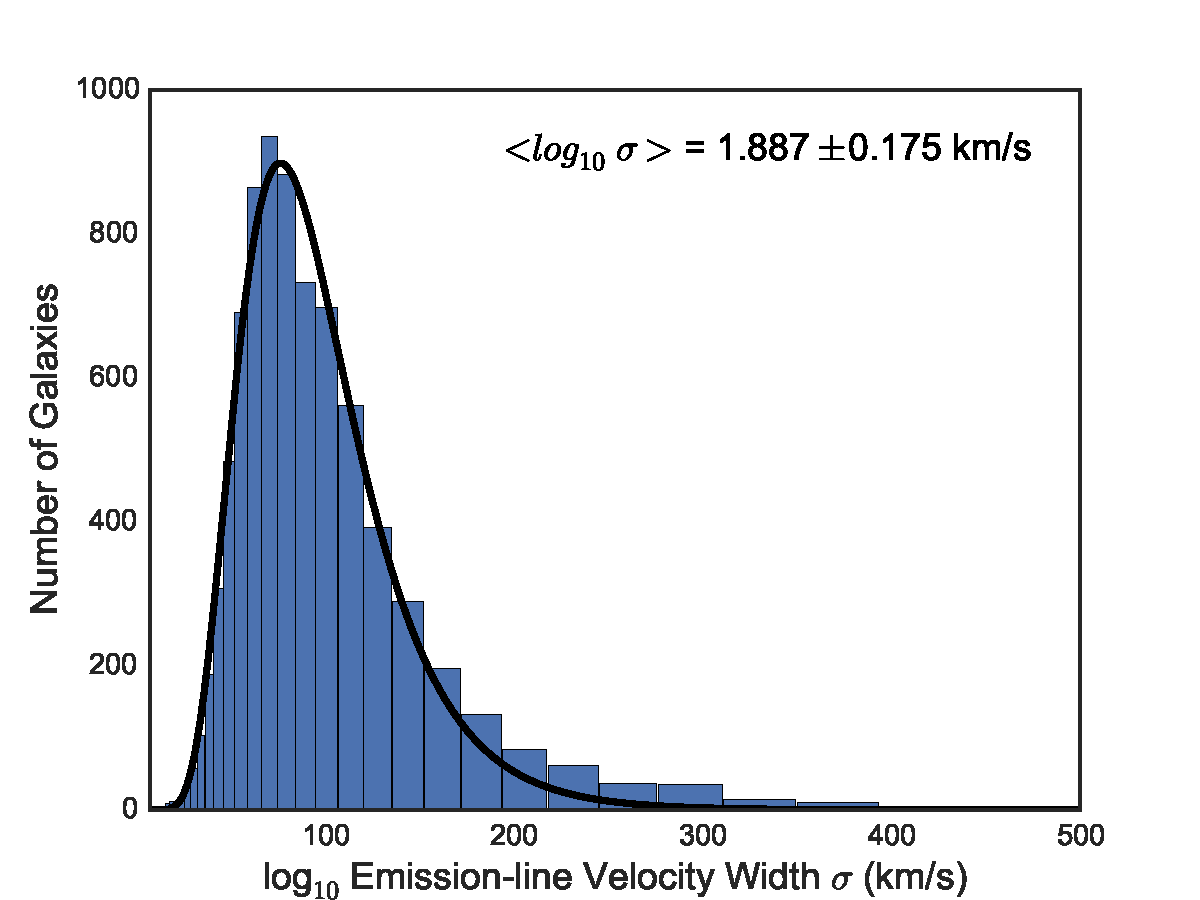
\includegraphics[width=0.8\textwidth]{figures/linesigma.pdf}
\caption{Distribution of emission-line velocity widths among DEEP2 galaxies at
  $z\sim1$.  The distribution is reasonably well-described by a log-normal
  distribution with mean and standard deviation of
  $\langle\log_{10}\sigma\rangle=1.877\pm0.175$~\kms{} or
  $\langle\sigma\rangle=77$~\kms.  \label{fig:linesigma}}
\end{figure}

\begin{figure}
\centering
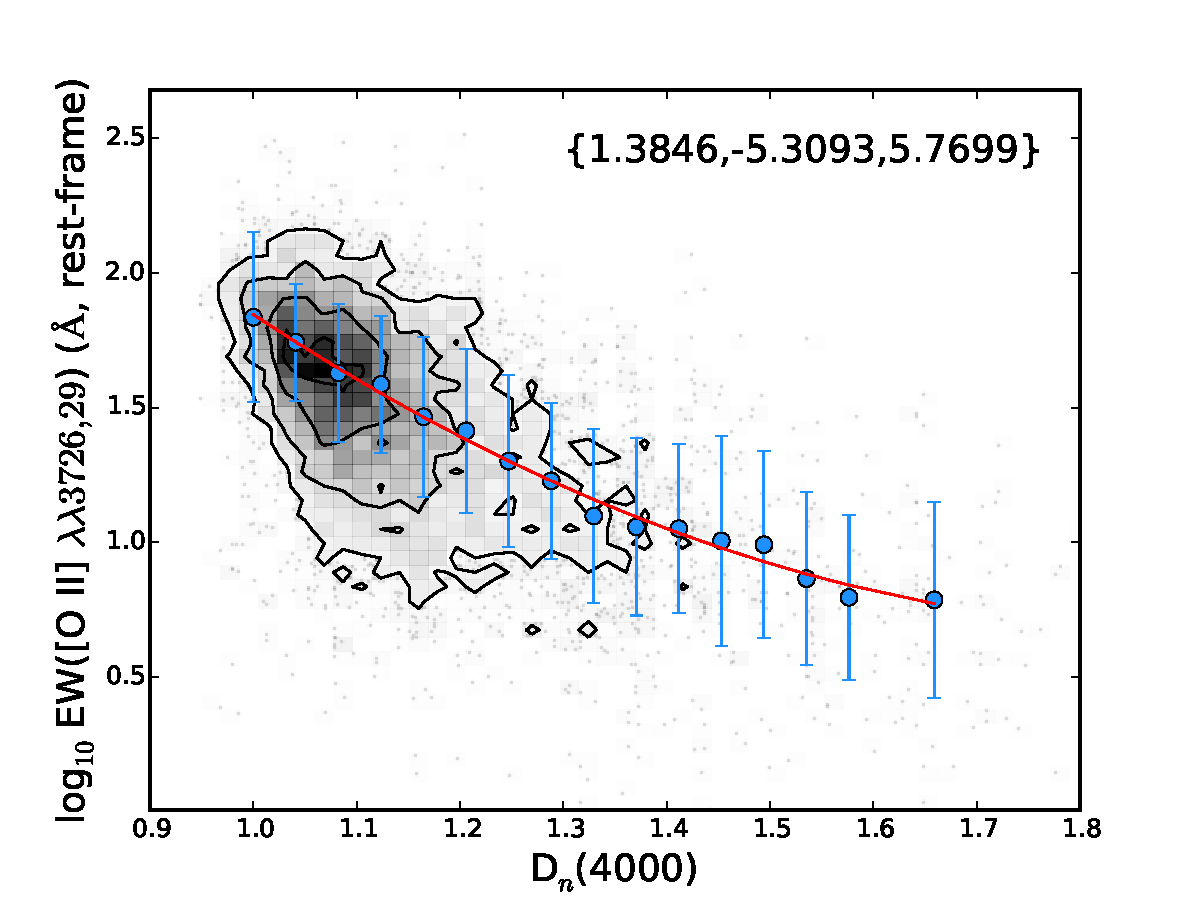
\includegraphics[width=0.8\textwidth]{figures/d4000_ewoii.pdf}
\caption{Rest-frame \oii{} equivalent width vs.~the $4000$-\AA{}
  break, $D_{n}(4000)$.  The blue points and uncertainties indicate
  the running median and standard deviation in $0.05$-wide bins of
  $D_{n}(4000)$, while the red curve is a third-order polynomial fit
  to the points with the coefficients given in the
  legend.  The dispersion is relatively uniform with $D_{n}(4000)$
  with a mean value of $0.30$~dex.  {\bf Show the subset of objects
    that satisfy our grz color cuts!}  \label{fig:d4000}}
\end{figure}

The ELG templates are constructed by combining the SEDs inferred from
modeling the broadband photometry with the \oii{} emission-line
profile and line-strength inferred from the DEEP2 spectroscopy.  The
script {\tt build\_desi\_elg\_templates} generates the actual ELG
templates from the parent sample of 35,682 DEEP2 galaxies.  First, a
subset of galaxies suitable for template-building are identified by
applying the following cuts:

\begin{enumerate}
\item[$\bullet$]{$0.75<z<1.45$;}
\item[$\bullet$]{$r_{\rm CFHTLS}<23.5$ (AB, extinction-corrected);}
\item[$\bullet$]{minimum 6 bands of observed-frame optical photometry;}
\item[$\bullet$]{\oiilam{} doublet measured with ${\rm S/N}>3$; and}
\item[$\bullet$]{EW(\oii)$>1$~\AA.}
\end{enumerate}

These cuts leave a total of $7876$ galaxies, the most stringent cut
being on the S/N of the \oii{} doublet.  Next, the \oii{} line-profile
and integrated flux for each galaxy is used as an anchor to construct
a more complete nebular emission-line spectrum.  Briefly, the nebular
emission-line model implemented within {\tt iSEDfit} is used to add
more than $50$ additional emission lines.  The strengths of the
hydrogen and helium recombination lines are based on the number of
hydrogen-ionizing photons inferred from the SED modeling, while the
forbidden emission-line strengths are based on empirically determined
line-ratios.

With these empirically constrained broadband SEDs and nebular
emission-line spectra in hand, a set of rest-frame and observed-frame
templates are generated.  

Tables~\ref{table:rest} and \ref{table:obs} summarize the spectral parameters of
the rest-frame and observed-frame templates, respectively.  The principle
difference between the two template sets is that the rest-frame templates have
constant-$\log_{10}(\lambda)$ ($20$~km~s$^{-1}$) pixels, while the
observed-frame templates have constant-$\lambda$ ($0.5$~\AA) pixels.  

In addition, the rest-frame templates are normalized to a $1~M_{\odot}$ (stellar
masss) stellar population at $10$~pc, while the observed-frame templates retain
the redshift and flux normalization of the corresponding DEEP2 galaxy.

%Include some figures:
%* color-redshift plots
%* many other ideas

\begin{enumerate}
\item{Extension~0: An [{\sc npixel}]$\times$[{\sc ntemplate}] flux
  array which contains {\sc ntemplate} spectra, each {\sc npixel}
  pixels long (see Table~\ref{table:rest} above).}
\item{Extension~1: An [{\sc ntemplate}] data structure with the
  following metadata:
\begin{itemize}
\item{.{\sc TEMPLATEID} - unique template ID number (zero-indexed)}
\end{itemize}
}
\end{enumerate}

The observed-frame template file, {\tt
  elg\_templates\_obs\_VERSION.fits.gz}, is a binary FITS table with
two extensions:

\begin{enumerate}
\item{Extension~0: An [{\sc npixel}]$\times$[{\sc ntemplate}] flux
  array which contains {\sc ntemplate} spectra, each {\sc npixel}
  pixels long (see Table~\ref{table:obs} above).}
\item{Extension~1: An [{\sc ntemplate}] data structure with the
  following metadata:
\begin{itemize}
\item{.{\sc TEMPLATEID} - unique template ID number (zero-indexed)}
\item{.{\sc OBJNO} - unique DEEP2 identifier}
\item{.{\sc RA} - right ascension (degrees, J2000)}
\item{.{\sc DEC} - declination (degrees, J2000)}
\item{.{\sc Z} - heliocentric redshift of the DEEP2 galaxy} 
\item{.{\sc SIGMA\_KMS} - intrinsic velocity line-width (km/s)} 
\item{.{\sc OII\_3726} - \oii~$\lambda3726$ emission-line flux
  (erg~s$^{-1}$~cm$^{^2}$)}  
\item{.{\sc OII\_3729} - \oii~$\lambda3729$ emission-line flux
  (erg~s$^{-1}$~cm$^{^2}$)} 
\item{.{\sc OII\_3727} - total \oiilam{} emission-line flux
  (erg~s$^{-1}$~cm$^{^2}$)} 
\item{.{\sc OII\_3727\_EW} - rest-frame \oii~$\lambda3726,29$
  equivalent width (\AA)}
\item{.{\sc RADIUS\_HALFLIGHT} - half-light radius (arcsec) ($-999$ if not measured)}
\item{.{\sc SERSICN} - Sersic n parameter (concentration) ($-999$ if not measured)}
\item{.{\sc AXIS\_RATIO} - minor-to-major axis ratio ($-999$ if not measured)}
\item{.{\sc DECAM\_G} - synthesized DECam g-band AB magnitude}
\item{.{\sc DECAM\_R} - synthesized DECam r-band AB magnitude}
\item{.{\sc DECAM\_Z} - synthesized DECam z-band AB magnitude}
\item{.{\sc LOGMSTAR} - log10(stellar mass) ($M_{\odot}$, $h=0.7$,
  \citealt{chabrier03a} IMF)} 
\item{.{\sc LOGSFR} - log10(star formation rate)
  ($M_{\odot}$~yr$^{-1}$, $h=0.7$, \citealt{chabrier03a} IMF)}
\item{.{\sc AV\_ISM} - $V$-band continuum attenuation (mag,
  \citealt{charlot00a} attenuation curve)} 
\end{itemize}
}
\end{enumerate}

\subsection{Luminous Red Galaxy (LRG) Templates} 


\subsection{Bright-Galaxy Survey (BGS) Templates} 

\subsection{Quasar (QSO) Templates }


\subsection{Stellar Templates (STAR)}


\subsection{Standard Stars (STD)}

\subsection{Future Improvements}

Future improvements to these templates may include (in no particular
order): 

\begin{enumerate}
\item{Extending the spectral coverage redward into the mid-infrared so
  that WISE photometry can be synthesized from the models.}
\item{Including additional nebular emission lines.}
\item{Constructing a smaller basis set of models (e.g., archetypes)
  which adequately span the physical parameter space of the full set
  of templates.}
\item{Incorporate more intelligent resampling of the data and models,
  in order to ensure that flux is being conserved correctly.}
\item{Expanding this TechNote to include more quantitative tests of
  the models (e.g., how well they span color-color and color-redshift
  space relative to actual observations).}
\end{enumerate}


\bibliographystyle{apj}
\bibliography{/Users/ioannis/bibdesk/ioannis}
%\input{elg-templates.bbl}


\clearpage
\appendix

\section{Installation Instructions}\label{sec:install}

First, be sure you have recent installations of the {\tt astropy} (needed to
manipulate FITS files), {\tt numpy} (numerical Python library), and {\tt
  matplotlib} (plotting library) packages, or install (or upgrade) them using
{\tt pip}:
\begin{itemize*}
  \item[\%]{{\tt pip install numpy [--upgrade]}}
  \item[\%]{{\tt pip install matplotlib [--upgrade]}}
  \item[\%]{{\tt pip install astropy [--upgrade]}}
\end{itemize*}

\noindent Next, clone the {\tt desihub/desisim}, {\tt desihub/desispec}, and
          {\tt desihub/imaginglss} repositories:
\begin{itemize*}
  \item[\%]{{\tt mkdir desihub ; cd desihub}}
  \item[\%]{{\tt git clone https://github.com/desihub/desisim.git}}
  \item[\%]{{\tt git clone https://github.com/desihub/desispec.git}}
  \item[\%]{{\tt git clone https://github.com/desihub/imaginglss.git}}
\end{itemize*}

\noindent The {\tt desispec} package is needed for the standardized set of I/O
routines which have been written for reading and writing DESI spectra (and the
associated metadata), while the {\tt imaginglss} package contains the DESI
target-selection algorithms.\footnote{Note that the target-selection criteria
  coded in {\tt imaginglss} eventually may be moved to the {\tt desitarget}
  product.}  Next, add these packages to your {\tt PYTHONPATH} environment.  For
example, in the {\tt bash} shell add the following lines to your {\tt .bashrc}
file:
\begin{itemize*}
  \item[\%]{{\tt DESIHUB=/path/to/desihub}}
  \item[\%]{{\tt
      PYTHONPATH=\$DESIHUB/desisim/py:\$DESIHUB/desispec/py:\$DESIHUB/imaginglss}}
\end{itemize*}

\noindent If you wish, create an alias which points to the top-level executable
script, {\tt simulate-templates.py}:
\begin{itemize*}
  \item[\%]{{\tt alias simulate-templates \$DESIHUB/desisim/bin/simulate-templates.py}}
\end{itemize*}

\noindent Finally, create environment variables which point to the latest set of
continuum (basis) spectra for each object type.  For example, on {\tt NERSC} you
would define the following variables in your {\tt .bashrc} startup file:
\begin{itemize*}
  \item[\%]{{\tt DESI\_ROOT=/project/projectdirs/desi}}
  \item[\%]{{\tt DESI\_TEMPLATES=\$DESI\_ROOT/spectro/templates}}
  \item[\%]{{\tt DESI\_ELG\_TEMPLATES=\$DESI\_TEMPLATES/elg\_templates/v1.3/elg\_templates\_v1.3.fits}}
  \item[\%]{{\tt DESI\_LRG\_TEMPLATES=\$DESI\_TEMPLATES/lrg\_templates/v1.1/lrg\_templates\_v1.1.fits}}
  \item[\%]{{\tt DESI\_BGS\_TEMPLATES=\$DESI\_TEMPLATES/bgs\_templates/v1.1/bgs\_templates\_v1.0.fits}}
  \item[\%]{{\tt DESI\_STAR\_TEMPLATES=\$DESI\_TEMPLATES/star\_templates/v1.1/star\_templates\_v1.1.fits}}
\end{itemize*}

\noindent Alternatively, you can transfer these binary FITS files to your local
machine or laptop and put them wherever you would like.  \noindent {\bf TODO:
  Write a test script which ensures everything has been properly
  installed/configured.}

\section{Tables of Nebular Emission Lines}

The following appendices do stuff.

\begin{deluxetable}{ccc}
\tablecaption{Nebular recombination lines\label{table:recomb}} 
\tablewidth{0pt}
\tablehead{\colhead{Emission Line} & \colhead{Vacuum Wavelength (\AA)} &
  \colhead{Ratio\tablenotemark{a}}} 
\startdata
Ly$\alpha$ & 1215.670 &    23.54656 \\
\cline{1-3}
H$\alpha$ & 6564.613 &    2.863158 \\
    H$\beta$ & 4862.683 &    1.000000 \\
   H$\gamma$ & 4341.684 &   0.4683401 \\
   H$\delta$ & 4102.892 &   0.2589474 \\
 H$\epsilon$ & 3971.195 &   0.1590283 \\
       H8 & 3890.151 &   0.1050202 \\
       H9 & 3836.472 &  0.07312550 \\
      H10 & 3798.976 &  0.05302830 \\
      H11 & 3771.701 &  0.03971660 \\
      H12 & 3751.217 &  0.03053440 \\
      H13 & 3735.430 &  0.02399190 \\
      H14 & 3722.997 &  0.01920650 \\
      H15 & 3713.027 &  0.01561130 \\
      H16 & 3704.906 &  0.01286640 \\
      H17 & 3698.204 &  0.01073680 \\
      H18 & 3692.605 & 0.009052600 \\
\cline{1-3}
  Pa$\alpha$ & 18756.13 &   0.3386235 \\
   Pa$\beta$ & 12821.59 &   0.1632389 \\
  Pa$\gamma$ & 10941.09 &  0.09044530 \\
  Pa$\delta$ & 10052.13 &  0.05545750 \\
Pa$\epsilon$ & 9548.591 &  0.03656680 \\
      Pa9 & 9231.547 &  0.02543320 \\
     Pa10 & 9017.385 &  0.01842910 \\
     Pa11 & 8865.217 &  0.01378950 \\
      P12 & 8752.876 &  0.01059920 \\
\cline{1-3}
  Br$\alpha$ & 40522.62 &  0.08021050 \\
   Br$\beta$ & 26258.67 &  0.04546560 \\
  Br$\gamma$ & 21661.20 &  0.02781380 \\
  Br$\delta$ & 19450.87 &  0.01825910 \\
\cline{1-3}
\hei~$\lambda3188$ & 3188.662 &  0.04076080 \\
\hei~$\lambda3389$ & 3889.752 &   0.1027011 \\
\hei~$\lambda3965$ & 3965.852 &  0.01022650 \\
\hei~$\lambda4026$ & 4027.348 &  0.02115760 \\
\hei~$\lambda4471$ & 4472.755 &  0.04445050 \\
\hei~$\lambda4922$ & 4923.304 &  0.01199870 \\
\hei~$\lambda5016$ & 5017.079 &  0.02568980 \\
\hei~$\lambda5876$ & 5877.299 &   0.1186800 \\
\hei~$\lambda6678$ & 6679.994 &  0.03360660 \\
\hei~$\lambda7065$ & 7067.198 &  0.02173860 \\
\hei~$\lambda10830$ & 10833.22 &   0.2404832
\enddata
\tablenotetext{a}{Ratio with respect to H$\beta$ assuming case~B recombination.} 
\end{deluxetable}

\begin{deluxetable}{cc}
\tablecaption{Nebular forbidden lines\label{table:forb}}
\tablewidth{0pt}
\tablehead{\colhead{Emission Line} & \colhead{Vacuum Wavelength (\AA)}}
\startdata
 \oii~$\lambda3726$ & 3727.092 \\
 \oii~$\lambda3729$ & 3729.874 \\
\oiii~$\lambda5007$ & 5008.239 \\
\oiii~$\lambda4959$ & 4960.295 \\
 \nii~$\lambda6584$ & 6585.277 \\
 \nii~$\lambda6548$ & 6549.852 \\
 \sii~$\lambda6716$ & 6718.294 \\
 \sii~$\lambda6731$ & 6732.673
\enddata
\end{deluxetable}

\end{document}


